\begin{question}[section=3,name={Feldbild},difficulty=,quantity=1,type=thr,tags={}]
	Skizzieren sie, wie das elektrische und das Magnetische Feld einer Parallelplattenleitung praktisch (d.h. ohne Idealisierung) aussieht! 
	\\ \textbf{Hinweis:}\\
	
\end{question}
\begin{solution}
	\begin{figure}[H]
		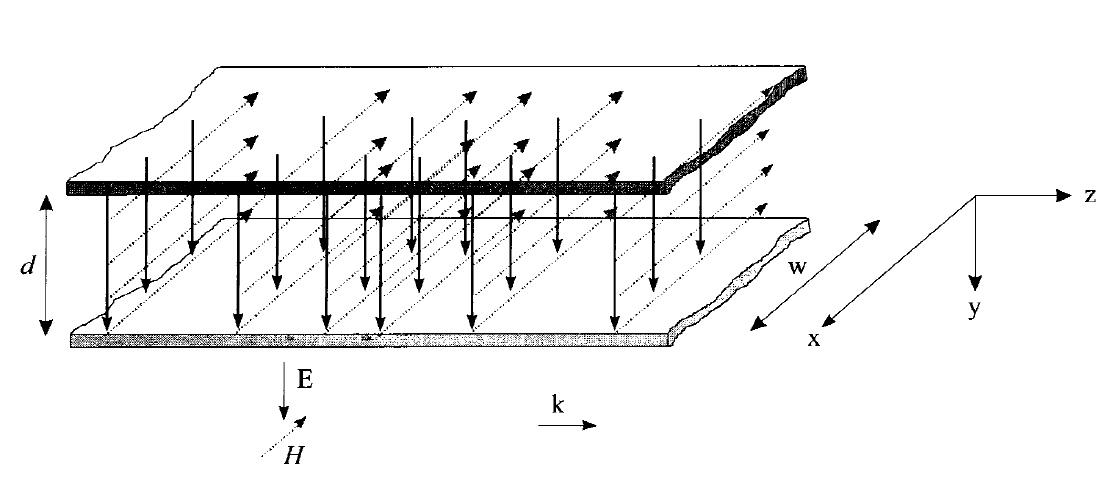
\includegraphics[width=14cm]{./opn/exm/thr/chp/3/1/bild.jpeg}
	\end{figure}
	Die Elektrischen Feldlinien schließen sich über den rechten und linken Raum.
\end{solution}